%
% chapter.tex -- Nichtkommutative harmonische Analysis
%
% (c) 2021 Prof Dr Andreas Müller, Hochschule Rapperswil
%
% !TeX spellcheck = de_CH
\chapter{Nichtkommutative harmonische Analysis
\label{buch:chapter:nichtkomm}}
\kopflinks{Nichtkommutative harmonische Analysis}

%
% 1-beispiele.tex
%
% (c) 2023 Prof Dr Andreas Müller, OST Ostschweizer Fachhochschule
%
\section{Beispiele
\label{buch:nichtkomm:section:beispiele}}
\kopfrechts{Beispiele}


%
% 2-unimodular.tex
%
% (c) 2022 Prof Dr Andreas Müller, OST Ostschweizer Fachhochschule
%
\section{Unimodularität
\label{buch:nichtkomm:section:unimodular}}
\kopfrechts{Unimodularität}

%
% 3-mittelung.tex
%
% (c) 2022 Prof Dr Andreas Müller, OST Ostschweizer Fachhochschule
%
\section{Mittelungsoperation
\label{buch:nichtkomm:section:mittelung}}
\kopfrechts{Mittelungsoperation}

%
% 4-gelfand.tex
%
% (c) 2022 Prof Dr Andreas Müller
%
\section{Charaktere und Gelfand-Transformation
\label{buch:gruppen:section:gelfand}}
\kopfrechts{Charaktere und Gelfand-Transformation}
In diesem Abschnitt suchen wir nach weiteren Möglichkeiten, einen
Zusammenhang zwischen der Algebra der Funktionen auf $G$ mit der Faltung
als Multiplikationsoperation und der Gruppe zu rekonstruieren.

%
% Charaktere der Faltungsalgebra
%
\subsection{Charaktere der Faltungsalgebra}
Die Faltung ist eine ziemlich komplizierte Operation.
Der Vektorraum der Funktionen auf $G$ ist ein unendlichdimensionaler
Vektorraum.
Die Unübersichtlichkeit der Faltung und die Dimension kann etwas
vorborgen werden, indem man komplexwertige Abbildungen untersucht,
die möglichst viel der Struktur erhalten.

\begin{definition}
Ein Vektorraum $A$ heisst {\em Algebra}, wenn aus auf $A$ eine bilineare
und assoziative Multiplikation $A\times A\to A$.
Wenn auf dem Vektorraunm $A$ ausserdem eine Norm definiert ist, dann
heisst $A$ eine normierte Algebra, wenn die Multiplikation die
Ungleichung
\[
\| xy \| \le \|x\|\cdot \|y\|\quad\text{für alle $x,y\in A$}.
\]
\end{definition}

\begin{definition}
Sei $A$ eine normierte Algebra.
Ein Charakter $\chi$ ist eine lineare Abbildung $\chi\colon A\to\mathbb{C}$,
die auch ein stetiger Algebrahomomorphismus ist, d.~h.~es gilt
$\chi(xy)=\chi(x)\chi(y)$.
\end{definition}

Als Beispiel betrachten wir den Vektorraum $C([a,b])$ der stetigen Funktionen
auf dem Intervall $[a,b]$ mit der Supremum Norm.
$C([a,b])$ ist aber auch eine Algebra, da Funktionen punktweise
multipliziert werden können.
Wenn $f,g\in C([a,b])$ zwei stetige Funktionen sind, dann ist
$fg\colon [a,b]\to\mathbb{C}:x\mapsto f(x)g(x)$ ein bilineares und
stetigs Produkt.
Für jeden Punkt $x\in[a,b]$ ist
\[
\chi_x
\colon
C([a,b] \to \mathbb{C}
:
f\mapsto f(x)
\]
eine stetige lineare Abbildung.
Sie ist aber auch ein Algebrahomomorphismus.
Dazu muss man nachrechnen, dass $\chi_x(fg)=\chi_x(f)\chi_y(f)$ ist.
Einsetzen der Definition von $\chi_x$ ergibt
\[
\chi_x(fg)
=
(fg)(x)
=
f(x)g(x)
=
\chi_x(f)\chi_x(g).
\]
Es gibt also zu jedem Punkt des Definitionsbereichs einen Charakter
der Algebra $C([a,b])$.

Man kann zeigen, dass die Homomorphismen von der Form $\chi_x$ 
die einzigen Homomorphismen $A\to\mathbb{C}$ sind.
Dies bedeutet, dass sich der Definitionsbereich der Algebra der
stetigen Funktionen vollständig aus der Algebra rekonstruiert werden 
kann.
Der Unterschied ist aber, dass die $[a,b]$ einfach nur eine Menge ist,
während $C([a,b])$ eine reichhaltige Algebrastruktur hat.

\begin{definition}
\label{buch:gruppen:gelfand:def:spektrum}
Ist $A$ eine Algebra, dann heisst die Menge
\[
\mathrm{X}(A)
=
\operatorname{Hom}(A,\mathbb{C})
\]
der Algebrahomomorphismen von $A$ nach $\mathbb{C}$ heisst das
{\em Spektrum} der Algebra $A$.
\end{definition}

Das Spektrum der Algebra der stetigen Funktionen auf einem Intervall
enthält die Charaktere $\chi_x$ mit $x\in [a,b]$, das Intervall
$[a,b]$ ist eine Teilmenge von $\mathbb{X}(C([a,b]))$.

%
% Homomorphismen G \to C^*
%
\subsection{Homomorphismen $G\to \mathbb{C}^*$}
Sei jetzt $G$ eine Gruppe mit einem Haarschen Mass und der Faltung 
von Funktionen mit kompaktem Träger.
Da die Funktionen alle in $L^2(G)$ drin sind, muss eine lineare
Abbildung nach dem Darstellungssatz von Riesz als ein Skalarprodukt
geschrieben werden können.
Für einen Charakter $\chi\colon L^2(G)\to\mathbb{C}$ muss es also eine
Funktion $\omega\colon G\to\mathbb{C}$ geben derart, dass
\begin{equation}
\langle \omega, f*g\rangle
=
\langle \omega, f\rangle
\langle \omega, g\rangle
\label{buch:gruppen:gelfand:eqn:omegahomo}
\end{equation}
gilt.
Aus dieser Bedingung lässt sich ableiten, dass $\omega$ sehr spezielle
Eigenschaften haben muss.

Seien $s,t\in G$ zwei Elemente der Gruppe.
Sei ausserdem $f$ eine Funktion, die nur in einer kleinen Umgebung 
des neutralen Elementes von $0$ verschieden ist.
Im Skalarprodukt
\[
\langle \omega, T_{s}f\rangle
=
\int_{G} \overline{\omega(x)} f(s^{-1}x) \,dx
\]
ist der Integrand nur für $x$ in unmittelbarer Nähe von $s$ 
$0$ verschieden.
Indem man die Funktion so verändert, dass der Träger kleiner wird,
dann konvergiert das Skalarprodukt gegen den Wert $\omega(s)$.
Aus \eqref{buch:gruppen:gelfand:eqn:omegahomo} folgt dann
\[
\omega(st) = \omega(s)\omega(t).
\]
Die Charaktere der Faltungsalgebra sind also genau die Homomorphismen
$G\mapsto\mathbb{C}^*$ von der Gruppe $G$ in die multiplikative
Gruppe von $\mathbb{C}$.

\begin{beispiel}
Sei $G= \mathbb{R}/2\pi\mathbb{Z}$ die Gruppe der Winkel mit der 
Addition von Winkeln als Gruppenoperation.
Um die Charaktere der Faltungsalgebra der $2\pi$-periodischen Funktionen
zu bestimmen, müssen Homomorphismen $G\to\mathbb{C}$ gefunden werden.
Ist $\omega$ ein solcher Homomorphismus, dann folgt aus
$h=\omega(\frac{2\pi}{n}$, $\omega(2\pi/n)^n = \omega(2\pi)=\omega(0)=1$.
Daher muss $h$ eine komplexe Zahl vom Betrag $1$ sein, die man als
$h=e^{it}$ schreiben kann.
Somit ist $\omega(2\pi k/n) = e^{ikt}$ eine Exponentialfunktion.
Da wir auch gefordert haben, das $\omega$ stetig sein muss folgt,
dass alle Homomorphismen von der Form $x\mapsto e^{ikx}$.
Da $\omega(2\pi)=1$ sein muss, folgt ausserdem, dass $k\in \mathbb{Z}$
ist.
Die Menge der Homomorphismen $G\to\mathbb{R}$ ist daher $\mathbb{Z}$ und
die Menge der Charaktere der Faltungsalgebra ist ebenfalls $\mathbb{Z}$.
\end{beispiel}


%
% Die Gelfand-Transformation
%
\subsection{Die Gelfand-Transformation}
Das Spektrum der Algebra $C([a,b])$ ist das Intervall $[a,b]$,
Es ist also möglich, aus der Algebra mit einer für alle Algebren
durchführbaren Prozedur eine Funktionenalgebra zu machen.
Den Funktionswert $f(x)$  kann man auch als Wert eines 
Algebrahomomorphismus $\chi_x(f) = f(x)$ bekommen.
Dies ist die Motivation für die folgende Definition.

\begin{definition}
Ist $A$ eine Algebra, dann ist die Gelfand-Transformation
die Abbildung
\[
\mathscr{G}
\colon
A \to C(\mathbb{X}(A))
:
a
\mapsto \mathscr{G}a = \hat{a}
\colon \chi \mapsto \hat{a}(\chi) = \chi(a).
\]
\end{definition}

\begin{satz}
Die Gelfand-Transformation ist ein Homomorphismus von Algebren.
\end{satz}

\begin{proof}
Es ist zu zeigen, dass $\mathscr{G}$ linear ist, ein Algebrahomomorphismus
und ausserdem stetig ist.
\begin{itemize}
\item
Linearität:
\begin{align*}
\mathscr{G}(\lambda a+\mu b) (\chi)
&=
\chi( \lambda a + \mu b)
=
\lambda\chi(a) + \mu\chi(b)
=
\lambda(\mathscr{G}a)(\chi)
+
\mu(\mathscr{G}b)(\chi)
\\
\Rightarrow\qquad
\mathscr{G}(\lambda a+ \mu b)
&=
\lambda\mathscr{G}a + \mu\mathscr{G}b.
\end{align*}
Somit ist $\mathscr{G}$ linear.
\item
Algebrahomomorphismus:
\begin{align*}
\mathscr{G}(ab)(\chi)
&=
\chi(ab)
=
\chi(a)\chi(b)
=
(\mathscr{G}a)(\chi)
(\mathscr{G}b)(\chi)
\\
\Rightarrow\qquad
\mathscr{G}(ab)
&=
\mathscr{G}a\cdot \mathscr{G}b.
\end{align*}
\item
\end{itemize}
\end{proof}

Sei jetzt $G$ eine Gruppe und $\mathscr{K}(G)$ die Algebra der
stetige Funktionen mit kompaktem Träger mit der Faltung.
Die Gelfand-Transformation macht aus einer Funktion auf $G$ 
eine Funktion auf dem Spektrum von $\mathscr{K}(G)$.
Ist $\chi\in\mathbb{X}(\mathscr{K}(G))$, dann hat die Gelfandtransformation
von $f\in\mathscr{K}(G)$ den Wert
\[
(\mathscr{G}f)(\chi) = \chi(f).
\]
Da die Gelfand-Transformatioin ein Algebrahomomorophismus ist,
muss  für jeden Homomorphismus $\chi$
\[
\mathscr{G}(f*g)(\chi)
=
(\mathscr{G}f\cdot \mathscr{G}g) (\chi)
=
\mathscr{G}f(\chi)
\mathscr{G}g(\chi)
\]
gelten.
Als Funktion auf $\mathbb{X}(\mathscr{K}(G))$ gilt für die
Gelfand-Transformtion daher
\[
\mathscr{G}(f*g)
=
\mathscr{G}f
\cdot
\mathscr{G}g,
\]
die Gelfand-Transformation macht also aus der Faltung die
gewöhnliche Multiplikation von Funktionen.

Für eine nichtabelsche Gruppe $G$ ist die Faltungsalgebra nicht
kommutativ.
Für zwei Funktionen $f$ und $g$ auf $G$ gilt jetzt aber
\[
\mathscr{G}(f*g)
=
\mathscr{G}f\cdot\mathscr{G}g
=
\mathscr{G}g\cdot\mathscr{G}f
=
\mathscr{G}(g*f).
\]
Die Gelfand-Transformation ignoriert also die Tatsache, dass im allgemeinen
$f * g\ne g*f$ ist.
Eine andere Möglichkeit, dies auszudrücken ist, dass der Kommutator
$f*g-g*f$ im Kern der Gelfand-Transformation liegt, also
\[
\mathscr{G}(f*g-g*f)=0.
\]

Wir wissen auch bereits, dass ein Algebrahomomorphismus
$\chi\colon \mathscr{K}(G)\to\mathbb{C}$ als Skalarprodukt mit
einem Gruppenhomomorphismus 
$\omega\colon G\to\mathbb{C}^*$ geschrieben werden kann.
Die Gelfand-Transformierte hat daher den Wert
\[
(\mathscr{G}f)(\chi)
=
\chi(f)
=
\langle \omega ,f\rangle
=
\int_G \overline{\omega(x)}\,f(x)\,dx.
\]

\begin{beispiel}
Für die Gruppe $\mathbb{R}/2\pi\mathbb{Z}$ der Winkel haben wir die
Menge der Homomorphismen bereits bestimmt, sie ist die Menge der
ganzen Zahlen $k\in\mathbb{Z}$ und der zugehörige Gruppenhomomorphismus
ist $\omega_k(x) = e^{ikx}$.
Die Gelfand-Transformation einer Funktion $f$ ist daher eine Funktion
auf den Zahlen $k\in \mathbb{Z}$ definiert durch
\[
(\mathscr{G}f)(k)
=
\hat{f}(k)
=
\langle \omega_k f\rangle
=
\int_{G/2\pi \mathbb{Z}} \overline{\omega_k(x)}\, f(x) \,dx
=
\int_0^{2\pi} \overline{e^{ikx}} f(x)\,dx
=
\int_0^{2\pi} e^{-ikx} f(x)\,dx.
\]
Die Werte der Fourier-Transformation auf $k\in\mathbb{Z}$ sind bis auf einen
Normierungsfaktor die Fourier-Koeffizienten der Funktion $f$.
\end{beispiel}

Die Gelfand-Transformation ist also eine Verallgemeinerung der
Fourier-Transformation, die automatisch auf eine Art von harmonischer
Analyse von Funktionen auf einer Gruppe führt.
Im Beispiel sind die Funktione $\omega_k$ bezüglich des
Skalarproduktes orthogonal, aber im Allgemeinen wissen wir dies 
noch nicht.
Wir werden in Abschnitt~\ref{buch:gruppen:section:darstellung}
auf diese Frage zurückkommen.



%
% Die duale Gruppe
%
\subsection{Die duale Gruppe}



%
% 5-mendez.tex
%
% (c) 2022 Prof Dr Andreas Müller, OST Ostschweizer Fachhochschule
%
\section{Méndez-Transformation
\label{buch:nichtkomm:section:mendez}}
\kopfrechts{Méndez-Transformation}
Die Mittelungsoperationen mit der Untergruppe $K\subset G$ ermöglichen,
Funktionen mit beliebigen Invarianzeigenschaften zu bekommen.
Die Theorie der Gelfand-Paare besagt, dass zwei Funktionen auf $X=G/K$
dadurch verglichen werden können, dass man zunächst die biinvarianten
Funktionen durch Linksmittelung konstruiert und dann diese beiden
vergleicht.
Stimmen die Funktionen überein, dann tun dies auch die gemittelten
Funktionen.
Aus dieser Idee lässt sich jetzt ein Werkzeug konstruieren, mit dem
das Registrierungsproblem vereinfacht werden kann.

%
% Verschiedene Einbettungen von K
%
\subsection{Verschiedene Einbettungen von $K$}
Die Gelfand-Theorie geht von $K$ als Untergruppe von $G$ aus und
konstruiert daraus die Algebra der biinvarianten Funktionen mit
der Faltung als Multiplikation.
Der Ausgangspunkt unserer Untersuchungen war aber der homogene
Raum $X$ mit der Operation $G$, der durch Auswahl eines Punktes $x\in X$
mit $G/S_x$ identifiziert worden ist.
Die Stabilisatoren $S_x$ sind alle isomorph zu $K$.
Die Wahl des Punktes $x\in X$ ist gleichbedeutend mit der Wahl einer
Einbettung der Gruppe $K$ in $G$.

Seien $f$ und $g$ zwei Funktionen auf $X$, die sich nur durch die
Translation mit einem Element $t\in G$ unterscheiden: $f(tx) = g(x)$.
Das Registrierungsproblem verlangt, $t$ zu finden.
Sei $x_1\in X$ ein beliebiger Punkt und $x_2=tx_1$.
Jedes andere Element $s$, welches $x_1$ auf $x_2$ abbildet,
also $x_2=sx_1$ erfüllt, liefert eine partielle Lösung
des Registrierungsproblems.
Die beiden Funktionen $f(sx)$ und $g(x)$ stimmen zwar im Punkt $x_1$
überein, aber ausserhalb dieses Punktes decken sie sich noch nicht.
Dazu ist die Anwendung eines Elementes des Stabilisators der
entsprechenden Funktionen notwendig.

Daraus lässt sich jetzt eine zweistufige Lösungsstrategie zur
Lösung des Registrierungsproblems ableiten.
Zunächst muss ein Paar von sich entsprechenden Punkten $x_2=tx_1$
der Funktionen $f$ und $g$ gefunden werden.
Die Translation der Funktion $f$ mit $t$ erreicht, dass die
beiden Funktionen in einem Punkt übereinstimmen.
Es muss dann nur noch ein Element von $S_{x_1}$ gefunden, mit
dem die beiden Funktionen vollends registriert werden können.

Der zweite Schritt in diesem Lösungsverfahren ist besonders einfach,
wenn $K$ eine abelsche Gruppe ist, wie dies im Falle der beiden
Registrierungsprobleme auf $S^2$ und $\mathbb{R}^2$ der Fall ist,
denn dazu kann die Fourier-Theorie verwendet werden.

%
% Die Méndez-Transformation
%
\subsection{Die Méndez-Transformation}
Der erste Schritt der oben vorgeschlagenen Lösungsansatzes verlangt,
dass man zu zwei Punkten $x_1,x_2\in X$ entscheiden können muss,
ob sie sich in den Funktionen $f$ und $g$ entsprechen.
Dazu kann man verwenden, sich nach einer Translation, die $x_1$ nach $x_2$
bringt, die Funktionen nur noch durch die Wirkung des Stabilisators
$S_{x_2}$ unterscheiden.
Mittelt man über die Wirkung von des Stabilisators, unterscheiden
sich die Funktionen gar nicht mehr.

Die Punkte $x_1$ und $x_2$ entsprechen sich also in den Funktionen $f$
und $g$ genau dann, wenn die über $S_{x_1}$ bzw.~$S_{x_2}$
gemittelten Funktionen übereinstimmen.
Sind die Funktionen $f$ und $g$ stetig, dann liegt $x_1$ nahe bei
dem Punkt, der $x_2$ entspricht, wenn die beiden gemittelten Funktionen
sich nur wenig unterscheiden.

\begin{definition}
Sie $G$ eine unimodulare lokalkompakte topologische Gruppe und $K$
eine kompakte Untergruppe und $f$ eine Funktion $G/K\to \mathbb{R}$.
Sei $\tilde{z}\in G$ ein Gruppenelement, das als Orbit
den Punkt $z\in K\backslash G/K$ hat.
Für jeden Punkt $x\in G/K$ ist dann die {\em Méndez-transformiert}
von $f$ definiert als
\[
(\mathcal{M}f)(x)(z)
=
\int_{S_x} f(k\tilde{z})\,dk
\]
der Mittelwert über die Orbits des Stabilisators von $x$.
\end{definition}

Die Méndez-Transformation mittelt also die Pixelwerte eines Bildes
über alle Orbits von $S_x$ und transportiert die Mittelwerte auf
den gemeinsamen Definitionsbereich $K\backslash G/K$, damit sie
verglichen werden können.

\begin{beispiel}
\begin{figure}
\centering
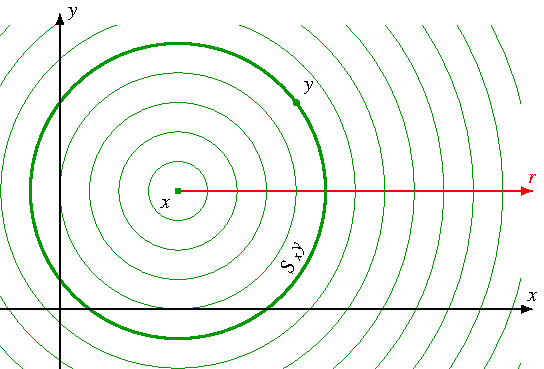
\includegraphics{chapters/070-nichtkomm/images/2dmendez.pdf}
\caption{Die Méndez-Transformation einer Funktion $f$ in der
Ebene an der Stelle $x,r$ ist der Mittelwert der Funktionswerte
auf auf dem Kreis $S_xy$ mit Radius $r=|y-x|$ um den Punkt $x$.
\label{buch:nichtkomm:mendez:fig:2d}}
\end{figure}
Für das Registrierungsproblem auf der Ebene mit der Gruppe
$\operatorname{SO}(2)\ltimes \mathbb{R}^2$ sind die Orbits des
Stabilisators eines Punktes $P=(x,y)$ Kreise vom Radius $r$ um
den Punkt (Abbildung~\ref{buch:nichtkomm:mendez:fig:2d}).
Der Raum $K\backslash G/K$ besteht aus den nichtnegativen
Zahlen $\mathbb{R}_{\ge 0}$.
Die Méndez-Transformation von $f$ hat daher die Werte
\[
\mathcal{M}f(P)(r)
=
\frac{1}{2\pi}
\int_0^{2\pi}
f(x+r\cos\varphi,y+r\sin\varphi)\,d\varphi.
\]
\end{beispiel}

\begin{beispiel}
\begin{figure}
\centering
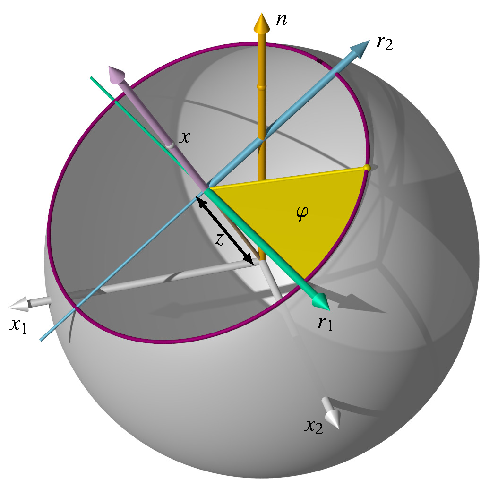
\includegraphics{chapters/070-nichtkomm/images/coordinates.pdf}
\caption{Koordinatensystem zur Berechnung der Méndez-Transformation
für das Paar $(G,K)=(\operatorname{SO}(3),\operatorname{SO}(2))$.
Die Koordinaten $z$ wird entlang der Achse mit Richtungsvektor $x\in S^2$
gemessen.
\label{buch:nichtkomm:mendez:fig:coordinates}}
\end{figure}
Für das Registrierungsproblem auf der Kugeloberfläche ist $x$ irgend ein
Einheitsvektor.
Die Orbits des Stabilisators von $x$ sind die Breitenkreise bezüglich
der Achse der Kugel durch $x$.
Sie sind durch die Höhe über der zu $x$ orthogonalen Äquatorebene der
Kugel charakterisiert.
Die Méndez-Transformierte einer Funktion $f\colon S^2\to \mathbb{R}$
an der Stelle $x$ ist daher eine Funktion $[-1,1]\to\mathbb{R}$ mit
dem Wert
\[
\mathcal{M}f (x)(z)
=
\int_{S_x} f(k\tilde{z})\,dk,
\]
wobei $\tilde{z}$ ein Einheitsektor mit $\tilde{z}\cdot x=z$ ist.
Das Integral ist der Mittelwert von $f$ über den Breitenkreis
auf Höhe $z$ um die Achse $x$.

In Abbildung~\ref{buch:nichtkomm:mendez:fig:coordinates} ist die
Achsrichtung $x\in S^2$ als hellvioletter Vektor eingezeichnet.
Die Koordinate $z\in[-1,1]$ wird vom Kugelmittelpunkt entlang dieser
Achse gemessen.
Zur Berechnung der Méndez-Transformation einer Funktion $f$ muss die
Funktion über den violett eingezeichneten Breitenkreis zur Achse $x$
integriert werden.
Dies kann mit Hilfe eines Integrals über den gelb eingezeichneten
Winkel $\varphi\in[0,2\pi]$ erfolgen.
Die Achsrichtungen $r_1=(n\times x)^0$ und $r_2=x\times r_1$ werden
aus der Richtung $n\in S^2$ des Nordpoles und $x$ berechnet.
Der Punkt mit Parameter $\varphi$ ist dann
\[
zx
+
\!\sqrt{1-z^2}(r_1 \cos\varphi + r_2 \sin\varphi).
\]
Die Méndez-Transformation kann damit als das Integral
\[
(\mathcal{M}f)(x)(z)
=
\frac{1}{2\pi}
\int_0^{2\pi}
f\left(
zx
+
\!\sqrt{1-z^2}(r_1 \cos\varphi + r_2 \sin\varphi)
\right)
d\varphi
\]
berechnet werden.
\end{beispiel}

Die Méndez-Transformation wurde von Tabea Méndez in 
\cite{buch:mendez} zur Lösung des Registrierungsproblems erfunden
und in \cite{buch:mendez-mueller} weiter verallgemeinert.
Die allgemeinste Darstellung der Theorie ist \cite[chapter 3]{buch:reg},
wo auch der Zusammenhang zur Radon-Transformation hergestellt wird.

%
% Lösung des Registrierungsproblems
%
\subsection{Lösung des Registrierungsproblems mit der Méndez-Transformation}
Es wurde bereits dargelegt, wie die Struktur des homogenen Raumes $G/K$
ermöglicht, das Registrierungsproblem in zwei einfachere Teilprobleme
zu zerlegen, nämlich das Finden eines Punktepaares, gefolgt von einem
Registrierungsproblem bezüglich der Gruppe $K$.
Mit der Méndez-Transformation kann der zweite Schritt jetzt vereinfacht
werden.
Wir zeigen hier nur das Prinzip, Optimierungsmöglichkeiten sind in
\cite{buch:mendez-mueller} und \cite{buch:reg} dargestellt.

%
% Registrierung mit einem Fixpunkt
%
\subsubsection{Registrierung mit einem Fixpunkt}
\begin{figure}
\centering
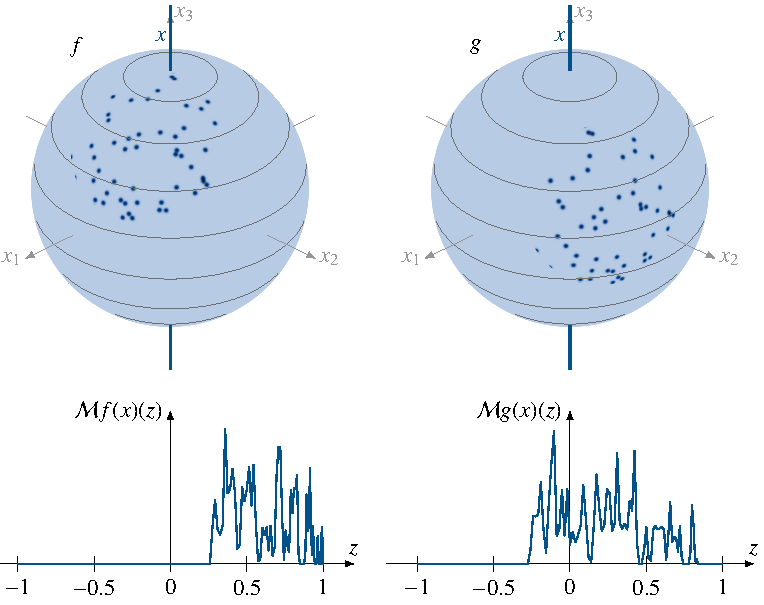
\includegraphics{chapters/070-nichtkomm/images/MTransformExamples.pdf}
\caption{Méndez-Transformation der zwei Funktionen $f$ und $g$ auf
der Kugeloberfläche.
Die $x_3$-Achse ist nicht die Drehachse der Drehung, die $f$ in $g$
überführt und die Méndez-Transformationen $\mathcal{M}f(x)$
und $\mathcal{M}g(x)$ sind klar verschieden.
\label{buch:nichtkomm:fig:mtex}}
\end{figure}
\begin{figure}
\centering
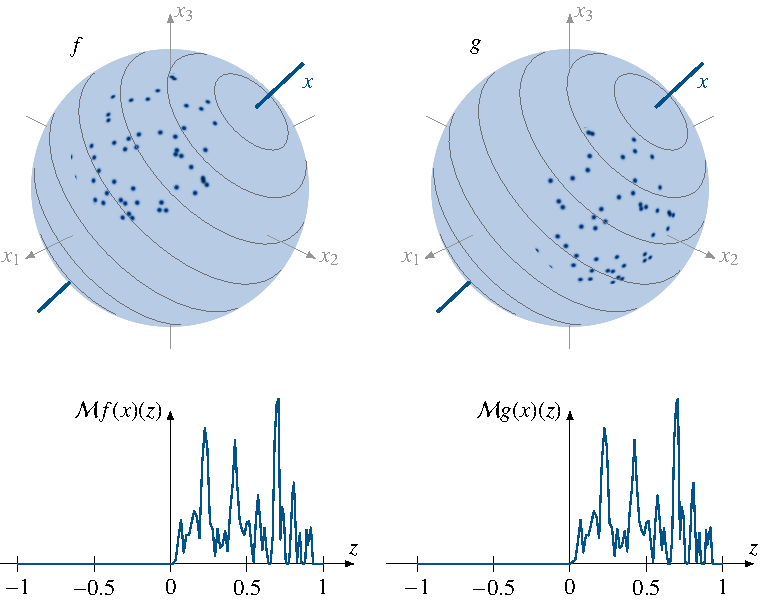
\includegraphics{chapters/070-nichtkomm/images/MTransformExamples2.pdf}
\caption{Méndez-Transformation der zwei Funktionen $f$ und $g$ auf
der Kugeloberfläche.
Die Achse mit Richtungsvektor $x$ gehört zu derjenigen Drehung,
die $f$ in $g$ überführt.
Die Méndez-Transformationen $\mathcal{M}f(x)$
und $\mathcal{M}g(x)$ sind gleich.
\label{buch:nichtkomm:fig:mtex2}}
\end{figure}
Falls die Wirkung der Gruppe $G$ auf $X$ immer einen Fixpunkt hat,
ist der erste Schritt des Registrierungsproblems besonders einfach
zu lösen.
In diesem Fall gibt es nämlich immer einen Punkt $x$, der beiden
Bildern gemeinsam ist.
Die Méndez-Transformationen $\mathcal{M}f(x)$ und $mathcal{M}g(x)$
sind daher die gleiche Funktion auf $Z=K\backslash G/K$.
Es muss daher nur der Definitionsbereich $X$ nach einem Punkt
durchsucht werden, für den $\mathcal{M}f(x) = \mathcal{M}g(x)$
gilt.
Da die Méndez-Transformation linear ist, bedeutet dies, dass nur
nach einer Nullstelle der Méndez-Transformation von $f-g$ gesucht
werden muss, also nach einem Punkt $x$, für den die Funktion
\(
\mathcal{M}(f-g)(x)
\)
die Nullfunktion ist.
Unter Berücksichtigung des Bildrauschens ist als $x$ so zu bestimmen,
dass die Norm $\| \mathcal{M}(f-g)(x) \|$ von $\mathcal{M}(f-g)(x)$
als Funktion auf $Z$ minimiert wird.

Das Registrierungsproblem auf der Kugeloberfläche gehört in diese
Klasse, den jede räumliche Drehung hat eine Drehachse, die fest
bleibt.
Das Finden eines Punktes mit $\mathcal{M}f(x)=\mathcal{M}g(x)$ 
kann immer noch eine ziemlich schwierige, nichtlineare Aufgabe sein.
Es ist aber nur noch ein zweidimensionales Problem, der Definitionsbereich
$S^2$ ist daher leichter zu durchsuchen als der dreidimensionale
Definitionsbereich $\operatorname{SO}(3)$.

Das Problem kann noch etwas vereinfacht werden durch die folgenden zwei
Beobachtungen, die in \cite{buch:mendez-mueller} etwas vertieft besprochen
werden.
\begin{enumerate}
\item
Für beliebige stetige Funktionen $f$ und $g$ ist die
Mendez-Transformation auch nur eine stetige Funktion und die
Abhängigkeit von $x$ ist im allgemeinen nicht differenzierbar.
Die Funktion $\|\mathcal{M}(f-g)(x)\|$ kann daher stark verrauscht
sein und es kann schwierig sein, das Minimum zu finden.
Durch Glättung der Funktionen kann erreicht werden, dass $f$ und $g$
differenzierbar sind, so dass das Minimum leichter zu finden ist.
\item
Glättung hat ausserdem den Vorteil, dass $x\mapsto\|\mathcal{M}(f-g)(x)\|_2^2$
eine differenzierbare Funktion ist, so dass ein gemäss 1.~gefundenes
approximatives Minimum mit Hilfe des quadratisch konvergenten Newtonschen
Algorithmus schnell verbessert werden kann.
\end{enumerate}

Weitere Möglichkeiten, die Lösung eines Registrierungsproblems mit
Hilfe eines Least-Squares-Ansatzes zu verbessern, sind in
\cite[chapter 3]{buch:reg} dargestellt.

%
% Registrierung ohne Fixpunkte
%
\subsubsection{Registrierung ohne Fixpunkte}
Beim Registrierungsproblem in der Ebene ist es möglich, dass die
Lösung ein reine Translation ist, die ausser im Fall der trivialen
Translation keine Fixpunkte hat.
In diesem Fall bleibt nichts anderes, als ein Punktepaar $x$ und $y$
zu finden so, dass $\mathcal{M}f(x)$ und $\mathcal{M}g(y)$ als Funktionen
auf $Z=K\backslash G/K$ übereinstimmen.
Dies sieht auf den ersten Blick nach einem sehr viel aufwendigeren
Problem aus, weil der Raum aller Punktepaare der vierdimensionale
Raum $\mathbb{R}^2\times\mathbb{R}^2$ ist.
Zwei Einschränkungen zeigen aber, dass dies nicht wirklich die
Schwierigkeit ist.
\begin{enumerate}
\item
Praktische Registrierungsprobleme suchen nur nach einer Translation
über eine beschränkte Distanz, gegeben durch die endliche Grösse 
der beiden Bilder.
\item
In einem realistischen Registrierungsproblem gibt es meistens einen
bekannten Bildpunkt des ersten Bildes, von dem man weiss, dass er auch
im zweiten Bild irgendwo vorkommt.
Es muss jetzt also nur noch der entsprechende Punkt im zweiten Bild
gesucht werden, was das Problem auf ein zweidimensionales Problem
reduziert.
\end{enumerate}




%
% 6-registrierung.tex
%
% (c) 2022 Prof Dr Andreas Müller, OST Ostschweizer Fachhochschule
%
\section{Registrierung
\label{buch:nichtkomm:section:registrierung}}
\kopfrechts{Registrierung}


%\section*{Übungsaufgaben}
%\rhead{Übungsaufgaben}
%\aufgabetoplevel{chapters/010-potenzen/uebungsaufgaben}
%\begin{uebungsaufgaben}
%\uebungsaufgabe{101}
%\uebungsaufgabe{102}
%\uebungsaufgabe{103}
%\uebungsaufgabe{104}
%\end{uebungsaufgaben}

